%%%%%%%%%%%%%%%%%%%%%%%%%%%%%%%%%%%%%%%%%
% University/School Laboratory Report
% LaTeX Template
% Version 3.1 (25/3/14)
%
% This template has been downloaded from:
% http://www.LaTeXTemplates.com
%
% Original author:
% Linux and Unix Users Group at Virginia Tech Wiki 
% (https://vtluug.org/wiki/Example_LaTeX_chem_lab_report)
%
% License:
% CC BY-NC-SA 3.0 (http://creativecommons.org/licenses/by-nc-sa/3.0/)
%
%%%%%%%%%%%%%%%%%%%%%%%%%%%%%%%%%%%%%%%%%

%----------------------------------------------------------------------------------------
%	PACKAGES AND DOCUMENT CONFIGURATIONS
%----------------------------------------------------------------------------------------

\documentclass{article}

\usepackage[utf8]{inputenc}
\usepackage{graphicx} % Required for the inclusion of images
%\usepackage{natbib} % Required to change bibliography style to APA
\usepackage{amsmath} % Required for some math elements 
\usepackage{glossaries}
\usepackage[toc,page]{appendix}
\usepackage[autostyle=true]{csquotes}
\usepackage{hyperref}
\usepackage{amssymb}
\usepackage{caption} 
\usepackage{hhline}
\usepackage{float}
\usepackage{listings}

\setlength\parindent{0pt} % Removes all indentation from paragraphs

%\usepackage{times} % Uncomment to use the Times New Roman font

%----------------------------------------------------------------------------------------
%	DOCUMENT INFORMATION
%----------------------------------------------------------------------------------------

\title{Reactive Agents:\\Functional Reactive Programming and ABM/S} % Title
 
\author{Jonathan \textsc{Thaler}} % Author name

\date{\today} % Date for the report

\begin{document}

\maketitle % Insert the title, author and date

% If you wish to include an abstract, uncomment the lines below
\begin{abstract}
In our previous work on update-strategies in Agent-Based Modelling \& Simulation (ABM/S) we showed that Haskell is a very attractive alternative to existing object-oriented approaches but our presented approach was too limited and we hypothesized that embedding it within a functional reactive framework like Yampa would leverage it to be able to build much more complex models. In this paper we investigate whether this hypothesis is true by testing if our approach can easily be transferred to Yampa, what we really gain from it and if more complex models can become reality. As a proof-of-concept we build a large, complex model from Agent-Based Computational Economics (ACE) which simulates the NASDAQ stock market.
\end{abstract}

\section{Introduction}
There exists a large number of simulation packages which allow the convenient creation of System Dynamics simulations by straight-forward visual diagram creation. One simply creates stocks and flows, connects them, specifies the flow-rates and initial parameters and then runs the model. An example for such a visual diagram creation in the simulation package AnyLogic can be seen in Figure \ref{fig:sir_stockflow_diagram}.

\begin{figure}
	\centering
	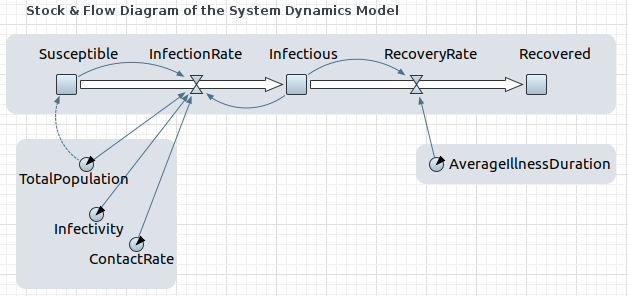
\includegraphics[width=.5\textwidth, angle=0]{./fig/SIR_SD_STOCKFLOW_DIAGRAMM.png}
	\caption{Visual System Dynamics Diagram of the SIR model in AnyLogic Personal Learning Edition 8.3.1.}
	\label{fig:sir_stockflow_diagram}
\end{figure}

Still, implementing System Dynamics directly in code is not as straight forward and involves numerical integration which can be quite tricky to get right. Thus, the aim of this paper is to look into how System Dynamics models can be implemented in code correctly without the use of a simulation package. We use the well known SIR model \cite{kermack_contribution_1927} from epidemiology to demonstrate our approach.

Our language of choice is Haskell because it emphasises a declarative programming style in which one describes \textit{what} instead of \textit{how} to compute. Further it allows to rule out interference with non-deterministic influences or side-effects already at compile-time. This is of fundamental importance for System Dynamics because it behaves completely deterministic and involves no stochastics or non-determinism whatsoever. Also, we make use of Functional Reactive Programming which allows to express continuous-time systems in a functional way. 

We show that by this approach we can arrive at correct-by-construction implementations of System Dynamic models. This means that the correctness of the code is obvious because we have closed the gap between the model specification and its implementation. Thus, the contribution of the paper is the demonstration of how to implement correct-by-construction System Dynamics simulations using Haskell and Functional Reactive Programming.

\section{Related Research}
Already noted in the Introduction, \cite{huberman_evolutionary_1993} where the first to discuss the differences update-strategies can make and introduced the terms of synchronous and asynchronous updates. They define to be synchronous as agents being updated in unison and asynchronous where one agent is updated and the others are held constant.

\medskip

\cite{a_framework_2008} give an approach for ABS on GPUs which is a very different approach to updating and iterating agents in ABS. They discuss execution order at length, highlight the problem of inducing a specific execution-order in a model which is problematic for parallel execution and give solutions how to circumvent these shortcomings. Although we haven't mapped our ideas to GPUs we explicitly include an approach for data-parallelism which, we hypothesize, can be utilized to roughly map their approach onto our terminology. 
	
\medskip
	
\cite{botta_time_2010} sketch a minimal ABS implementation in Haskell which is very similar in the basic structure of ours. This proves that our approach seems to be a very natural one to apply to Haskell. Their focus is primarily on economic simulations and instead of iterating a simulation with a global time, their focus is on how to synchronize agents which have internal, local transition times. Although their work uses Haskell as well, our focus is very different from theirs and approaches ABS in a more general and comprehensive way.

\medskip

\cite{dawson_opening_2014} describe basic inner workings of ABS environments and compare their implementation in C++ to the existing ABS environment AnyLogic which is programmed in Java. They explicitly mention asynchronous and synchronous time-models and compare them in theory but unfortunately couldn't report the results of asynchronous updates due to limited space. They interpret asynchronous time-models to be the ones in which an agent acts at random time intervals and synchronous time-models where agents are updated all in same time intervals.

\medskip

\cite{yuxuan_agent-based_2016} presents in his Master-Thesis a comprehensive discussion on how to implement an ABS for state-charts in Java and also mentions synchronous and asynchronous time-models. He identifies the asynchronous time-model to be one in which updates are triggered by the exchange of messages and the synchronous ones which trigger changes immediately without the indirection of messages.

\medskip

We observe that there seems to be a variety of meanings attributed to the terminology of asynchronous and synchronous updates but the very semantic and technical details are unclear and not described very precisely. In the next section we will address this issue by presenting the basic background and propose properties for a new terminology from which we can derive common update-strategies.

\section{The Problem}

ABM/S is a method of modelling and simulating a system where the global behaviour may be unknown but the behaviour and interactions of the parts making up the system is of knowledge \cite{wooldridge_introduction_2009}. Those parts, called Agents, are modelled and simulated out of which then the aggregate global behaviour of the whole system emerges. Thus the central aspect of ABM/S is the concept of an Agent which can be understood as a metaphor for a unique pro-active unit, able to spawn new Agents, interacting with other Agents in a network of neighbours by exchange of messages which are situated in a generic environment. Thus we informally assume the following about our Agents:

\begin{itemize}
	\item They have a unique identifier
	\item They can initiate actions on their own e.g. change their own state, send messages, create new agents, kill themselves,...
	\item They can react to messages they receive with actions (see above)
	\item They can interact with a generic environment they are situated in
\end{itemize} 

An implementation of an ABS must solve thus solve three fundamental problems:
\begin{enumerate}
	\item Source of pro-activity \\ How can an Agent initiate actions without external stimuli?
	\item Message-Processing \\ When is a message \textit{m}, visible to Agent \textit{B}, processed by it?
	\item Semantics of Message-Delivery \\ When is a message \textit{m}, sent by Agent \textit{A} to Agent \textit{B}, visible to \textit{B}?
\end{enumerate}

In computer systems, pro-activity, the ability to initiate actions on its own without external stimuli, is only possible when there is some internal stimuli, most naturally represented by some generic notion of monotonic increasing time-flow. This can either be some physical real-time system-clock which counts the milliseconds since 1970 (thus binding the time-flow of the system to the one of the 'real-world') or a virtual simulation-clock which is just a monotonic increasing natural number. As we are in a discrete computer-system, this time-flow must be discretized as well in discrete steps and each step must be made available to the Agent, acting as one internal stimuli. This allows the Agent then to perceive time and become pro-active depending on time (NOTE: we could argue that this is not really pro-activity because it depends always on time, but there is really now other way of doing this in our current implementation of computer-systems.). Independent of the representation of the time-flow we have the two fundamental choices whether the time-flow is local to the Agent or whether it is a system-global time-flow.

\medskip 

The semantics of message-delivery define when sent messages are visible to the receivers so they can process them and react to them. The only two ways of implementing them are that messages are visible either \textit{immediately} or after a synchronization point between the sender and receiver. Such a synchronization point can be a local one, just between the two or a global one between all Agents in the system.

\medskip 

Basically we can say that we want to process a message as soon as it is visible to us but this is not how real computer-systems can work. In a real system each Agent would have a message-box into which the messages are posted so the Agent can then check its mail-box for new messages. The question is then when the Agent is going to poll for new messages? Clearly what we need is a recurring, regular trigger which allows the Agent to poll the mail-box and process all queued messages. We argue that the most natural approach is to bind this trigger to the time-flow step which provides pro-activity.

\medskip 

To solve these problems an update-strategy is implemented which will iterate through the Agents in \textit{some} way and allow the Agents to perform these steps. It is immediately clear that different choices in the specific problems will lead to different system behaviour. To discuss this we will first present all possible update-strategies and their details in the next section and then outline how they influence the system behaviour.

\section{FRP and Yampa}
2 Pages

\section{Results}

\graphicspath{{./fig/}}	%specifying the folder for the figures

The coordinates calculated by the agents are \textit{virtual} ones ranging between 0.0 and 1.0. This prevents us from knowing the rendering-resolution and polluting code which has nothing to do with rendering with these implementation-details. Also this simulation could run without rendering-output or any rendering-frontend thus sticking to virtual coordinates is also very useful regarding this (but then again: what is the use of this simulation without any visual output=


\subsection{Reasoning}
Allowing to reason about a program is one of the most interesting and powerful features of a Haskell-program. Just by looking at the types one can show that there is no randomness in the simulation \textit{after} the random initialization, which is not slightest possible in the case of a Java, Scala, ReLogo or NetLogo solution. Things we can reason about just by looking at types:

\begin{itemize}
\item Concurrency involved?
\item Randomness involved?
\item IO with the system (e.g. user-input, read/write to file(s),...) involved?
\item Termination?
\end{itemize}

This all boils down to the question of whether there are \textit{side-effects} included in the simulation or not.

What about reasoning about the termination? Is this possible in Haskell? Is it possible by types alone? My hypothesis is that the types are an important hint but are not able to give a clear hint about termination and thus we we need a closer look at the implementation. In dependently-typed programming languages like Agda this should be then possible and the program is then also a 
proof that the program itself terminates.

reasoning about Heros \& Cowards: what can we deduce from the types? what can we deduce from the implementation?\\

Compare the pure-version (both Yampa and classic) with the IO-version of haskell: we loose basically all power to reason by just looking at the types as all kind of side-effects are possible when running in the IO-Monad.

in haskell pure version i can guarantee by reasoning and looking at the types that the update strategy will be simultaneous deterministic. i cant do that in java

TODO: implement haskell-version with shared-state (STM primitives) without using IO
TODO: implement haskell-version which defines abstract types for the simulation


\subsubsection{The type of a Simulation}
the type of a simulation: try to define the most general types of a simulation and then do reasoning about it

simulation :: Model -> Double -> Int -> [Model]

step :: Model -> Double -> Model

TODO: can we say something about the methods Model can/must/should support?

\subsection{Debugging \& Testing}
Because functions compose easier than classes \& objects (TODO: we need hard claims here, look for literature supporting this thesis or proof it by myself) it is also much easier to debug \textit{parts} of the implementation e.g. the rendering of the agents without any changes to the system as a whole - just the main-loop has do be adopted. Then it is very easy to calculate e.g. only one iteration and to freeze the result or to manually create agents instead of randomly create initial ones.

TODO: quickcheck \cite{claessen_quickcheck:_2000}


\subsection{Lazy Evaluation}
can specify to run the simulation for an unlimited number of steps but only the ones which are required so far are calculated.

\subsection{Performance}
Java outperforms Haskell implementation easily with 100.000 Agents - at first not surprising because of in-place updates of friend and enemies and no massive copy-overhead as in haskell. But look WHERE exactly we loose / where the hotspots are in both solutions. 1000.000 seems to be too much even for the Java-implementation.

\subsection{Numerical Stability}
The agents in the Java-implementation collapsed after a given number of iterations into a single point as during normalization of the direction-vector the length was calculated to be 0. This could be possible if agents come close enough to each other e.g. in the border-worldtype it was highly probable after some iterations when enough agents have assembled at the borders whereas in the Wrapping-WorldType it didn't occur in any run done so far. \\
In the case of a 0-length vector a division by 0  resulting in NaN which \textit{spread} through the network of neighbourhood as every agent calculated its new position it got \textit{infected} by the NaN of a neighbour at some point. The solution was to simply return a 0-vector instead of the normalized which resulted in no movement at all for the current iteration step of the agent. 


\subsection{Update-Strategies}
\begin{enumerate}
\item All states are copied/frozen which has the effect that all agents update their positions \textit{simultaneously}
\item Updating one agent after another utilizing aliasing (sharing of references) to allow agents updated \textit{after} agents before to see the agents updated before them. Here we have also two strategies: deterministic- and random-traversal.
\item Local observations: Akka
\end{enumerate}

\subsection{Different results with different Update-Strategies?}
Problem: the following properties have to be the same to reproduce the same results in different implementations: \\

Same initial data: Random-Number-Generators
Same numerical-computation: floating-point arithmetic
Same ordering of events: update-strategy, traversal, parallelism, concurrency

\begin{itemize}
\item Same Random-Number Generator (RNG) algorithm which must produce the same sequence given the same initial seed.
\item Same Floating-Point arithmetic
\item Same ordering of events: in Scala \& Actors this is impossible to achieve because actors run in parallel thus relying on os-specific non-deterministic scheduling. Note that although the scheduling algorithm is of course deterministic in all os (i guess) the time when a thread is scheduled depends on the current state of the system which can change all the time due to \textit{very} high number of variables outside of influence (some of the non-deterministic): user-input, network-input, .... which in effect make the system appear as non-deterministic due to highly complex dependencies and feedback.
\item Same dt sequence => dt MUST NOT come from GUI/rendering-loop because gui/rendering is, as all parallelism/concurency subject to performance variations depending on scheduling and load of OS.
\end{itemize}

It is possible to compare the influences of update-strategies in the Java implementation by running two exact simulations (agentcount, speed, dt, herodistribution, random-seed, world-type) in lock-step and comparing the positions of the agent-pairs with same ids after each iteration. If either the x or y coordinate is no equal then the positions are defined to be \textit{not} equal and thus we assume the simulations have then diverged from each other. \\
It is clear that we cannot compare two floating-point numbers by trivial == operator as floating-point numbers always suffer rounding errors thus introducing imprecision. What may seem to be a straight-forward solution would be to introduce some epsilon, measuring the absolute error: abs(x1 - x2) > epsilon, but this still has its pitfalls. The problem with this is that, when number being compared are very small as well then epsilon could be far too big thus returning to be true despite the small numbers are compared to each other quite different. Also if the numbers are very large the epsilon could end up being smaller than the smallest rounding error, so that this comparison will always return false. The solution would be to look at the \textit{relative error}: abs((a-b)/b) < epsilon. \\
The problem of introducing a relative error is that in our case although the relative error can be very small the comparison could be determined to be different but looking in fact exactly the same without being able to be distinguished with the eye. Thus we make use of the fact that our coordinates are virtual ones, always being in the range of [0..1] and are falling back to the measure of absolute error with an epsilon of 0.1. Why this big epsilon? Because this will then definitely show us that the simulation is \textit{different}. \\

The question is then which update-strategies lead to diverging results. The hypothesis is that when doing simultaneous updates it should make no difference when doing random-traversal or deterministic traversal => when comparing two simulations with simultaneous updates and all the same except first random- and the other deterministic traversal then they should never diverge. Why? Because in the simultaneous updates there is no ordering introduce, all states are frozen and thus the ordering of the updates should have no influence, \textit{both simulations should never diverge, \textbf{independent how dt and epsilon are selected}}. \\
Do the simulation-results support the hypothesis? Yes they support the hypothesis - even in the worst cast with very large dt compared to epsilon (e.g. dt = 1.0, epsilon = 1.0-12)

The 2nd hypothesis is then of course that when doing consecutive updates the simulations will \textit{always} diverge independent when having different traversal-strategies. \\
Simulations show that the selection of \textit{dt} is crucial in how fast the simulations diverge when using different traversal-strategies. The observation is that \textit{The larger dt the faster they diverge and the more substantial and earlier the divergence.}. Of course it is not possible to proof using simulations alone that they will always diverge when having different traversal-strategies. Maybe looking at the dynamics of the error (the maximum of the difference of the x and y pairs) would reveal some insight? \\

The 3rd hypothesis is that the number of agents should also lead to increased speed of divergence when having different traversal-strategies. This could be shown when going from 60 agents with a dt of 0.01 which never exceeded a global error of 0.02 to 6000 agents which after 3239 steps exceeded the absolute error of 0.1.

\subsection{Reproducing Results in different Implementations}
actors: time is always local and thus information as well. if we fall back to a global time like system time we would also fall back to real-time. anyway in distributed systems clock sync is a very non-trivial problem and inherently not possible (really?). thus using some global clock on a metalevel above/outside the simulation will only buy us more problems than it would solve us. real-time does not help either as it is never hard real time and thus also unpredictable: if one tells the actor to send itself a message after 100ms then one relies on the capability of the OS-timer and scheduler to schedule exactly after 100ms: something which is always possible thus 100ms are never hard 100ms but soft with variations.

qualitative comparison: print pucture with patterns. all implementations are able to reproduce these patterns independent from the update strategy

no need to compare individual runs and waste time in implementing RNGs, what is more interesting is whether the qualitative results are the same: does the system show the same emergent behaviour? Of course if we can show that the system will behave exactly the same then it will also exhibit the same emergent behaviour but that is not possible under some circumstances e.g. the simulation-runs of Akka are always unique and never comparable due to random event-ordering produced by concurrency \& scheduling. Also we don't have to proof the obvious: given the same algorithm, the same random-data, the same treatment of numbers and the same ordering of events, the outcome \textit{must} be the same, otherwise there are bugs in the program. Thus when comparing results given all the above mentioned properties are the same one in effect tests only if the programs contain no bugs - or the same bugs, if they \textit{are the same}. \\

Thus we can say: the systems behave qualitatively the same under different event-orderings.

Thus the essence of this boils down to the question: "Is the emergent behaviour of the system is stable under random/different/varying event-ordering?". In this case it seems to be so as proofed by the Akka implementation. In fact this is a very desirable property of a system showing emergent behaviour but we need to get much more precise here: what is an event? what is an emergent behaviour of a system? what is random-ordering of events? (Note: obviously we are speaking about repeated runs of a system where the initial conditions may be the same but due to implementation details like concurrency we get a different event-ordering in each simulation-run, thus the event-orderings vary between runs, they can be in fact be regarded as random).

\begin{figure}[H]
	\centering
  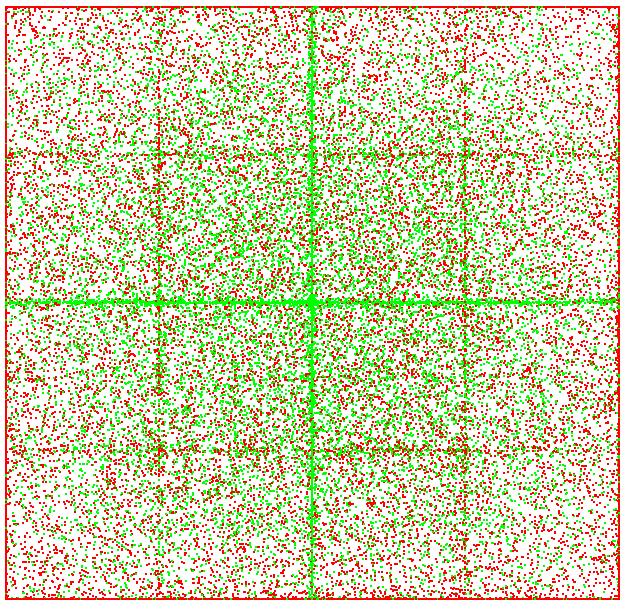
\includegraphics[width=1.0\textwidth, angle=0]{EMERGENT_PATTERN.png}
  	\caption{The emergent pattern used as criteria for qualitative comparison of implementations. Note the big green cross in the center and the smaller red crosses in each sub-sector. World-type is \textit{border} with 100.000 Agents where 25\% are Heroes.}
	\label{fig:EMERGENT_PATTERN}
\end{figure}


\subsection{Problem of RNG}
Have to behave EXACTLY The same: VERY difficult because of differing interfaces e.g. compare java to haskell RNGs.
Solution: create a deterministic RNG generating a number-stream starting from 1 and just counting up. The program should work also in this case, if not, something should be flawed!

Peer told me to implement a RNG-Trace: generate a list of 1000.0000 pre-calculated random-numbers in range of [0..1], store them in a file and read the trace in all implementations. Needs lots of implementation.

\subsection{Run-Time Complexity}
what if the number of agents grows? how does the run-time complexity of the simulation increases? Does it differ from implementation to implementation? The model is O(n) but is this true for the implementation?

\subsection{Simulation-Loops}
There are at least 2 parts to implementing a simulation: 1. implementing the logic of an agent and 2. implementing the iteration/recursion which drives the whole simulation

Classic \\
Yampa \\ TODO: use par to parallelize
Gloss \\
gloss provides means for simple simulation using simulate method. But: are all ABM systems like that?

\subsection{Agent-Representation}
Java: (immutable) Object
Haskell Classic: a struct
Haskell Yampa: a Signal-Function
Gloss: same as haskell classic
Akka: Actors

\subsection{EDSL}
simplify simulation into concise EDSL: distinguish between different kind if sims: continuous/discrete iteration on: fixed set, growing set, shrinking set, dynamic set. 

\section{Conclusion and further research}

So far we only looked at recursive simulation in a simulation with a strictly sequential update-strategy where agents are updated in sequence after each other as defined in TODO: cite my Art-Of-Iteration Paper. We leave the question of how Meta-ABS would apply to the parallel update-strategy and whether it is reasonable to extend it to that strategy or not for further research.

Research Questions
\begin{enumerate}
	\item How does deep regression influence the dynamics of a system? Hypothesis: TODO
	\item How do the dynamics of a system change when using perfect information or learning local information? Hypothesis: TODO
	\item Is a hidden markov model suitable for the local learning? Hypothesis: TODO
	\item How can MetaABS best be implemented? Hypothesis: implementing a MetaABS EDSL in a pure functional language like Haskell, should be best suited due to its inherent recursive, declarative nature, which should allow a direct mapping of features of this paradigm to the specification of the meta-model
\end{enumerate}

Problems
\begin{itemize}
	\item Definition of a recursive, declarative description of the Model.
	\item Perfect information about other agents is not realistic and runs counter to agent-based simulation (especially in social sciences) thus an Agent needs to be able to have local, noisy representations of the other agents.
	\item Local representation of other agents could be captured by Hidden Markov Models: observe what other agents do but have hidden interpretation of their internal state - these internal state-representations can be different between the local and the global version whereas the agent learns to represent the global version as best as possible locally.
	\item Infinite regress is theoretically possible but not on computers, we need to terminate at some point
\end{itemize}

\section{Further Research}
\label{sec:further_research}
We see this paper as an intermediary and necessary step towards dependent types for which we first needed to understand the potential and limitations of a non-dependently typed pure functional approach in Haskell. Dependent types are extremely promising in functional programming as they allow us to express stronger guarantees about the correctness of programs and go as far as allowing to formulate programs and types as constructive proofs which must be total by definition \cite{thompson_type_1991, mckinna_why_2006, altenkirch_pi_2010}.

So far no research using dependent types in agent-based simulation exists at all. In our next paper we want to explore this for the first time and ask more specifically how we can add dependent types to our pure functional approach, which conceptual implications this has for ABS and what we gain from doing so. We plan on using Idris \cite{brady_idris_2013} as the language of choice as it is very close to Haskell with focus on real-world application and running programs as opposed to other languages with dependent types e.g. Agda and Coq which serve primarily as proof assistants.

We hypothesize that dependent types could help ruling out even more classes of bugs at compile time and encode invariants and model specifications on the type level, which implies that we don't need to test them using e.g. property-testing with QuickCheck. This would allow the ABS community to reason about a model directly in code. We think that a promising approach is to follow the work of \cite{brady_correct-by-construction_2010, brady_idris_2011, brady_programming_2013, fowler_dependent_2014, brady_state_2016} in which the authors utilize GADTs to implement an indexed monad which allows to implementation correct-by-construction software.

\begin{itemize}
% NOTE: ran out of space
%	\item Accessing the environment in section \ref{sec:adding_env} involves indexed array access which is always potentially dangerous as the indices have to be checked at run-time. Using dependent types it should be possible to encode the environment dimensions into the types. In combination with suitable data types for coordinates one should be able to ensure already at compile time that access happens only within the bounds of the environment.

	\item In the SIR implementation one could make wrong state-transitions e.g. when an infected agent should recover, nothing prevents one from making the transition back to susceptible. 
	
	Using dependent types it should be possible to encode invariants and state-machines on the type level which can prevent such invalid transitions already at compile time. This would be a huge benefit for ABS because many agent-based models define their agents in terms of state-machines.
	
	\item An infected agent recovers after a given time - the transition of infected to recovered is a timed transition. Nothing prevents us from \textit{never} doing the transition at all. 
	
	With dependent types we should be able to encode the passing of time in the types and guarantee on a type level that an infected agent has to recover after a finite number of time steps.
	
	\item In more sophisticated models agents interact in more complex ways with each other e.g. through message exchange using agent IDs to identify target agents. The existence of an agent is not guaranteed and depends on the simulation time because agents can be created or terminated at any point during simulation. 
	
	Dependent types could be used to implement agent IDs as a proof that an agent with the given id exists \textit{at the current time-step}. This also implies that such a proof cannot be used in the future, which is prevented by the type system as it is not safe to assume that the agent will still exist in the next step.

	\item In our implementation, we terminate the SIR model always after a fixed number of time-steps. We can informally reason that restricting the simulation to a fixed number of time-steps is not necessary because the SIR model \textit{has to} reach a steady state after a finite number of steps. This means that at that point the dynamics won't change any more, thus one can safely terminate the simulation. Informally speaking, the reason for that is that eventually the system will run out of infected agents, which are the drivers of the dynamic. We know that all infected agents will recover after a finite number of time-steps \textit{and} that there is only a finite source for infected agents which is monotonously decreasing. 
	
	Using dependent types it might be possible to encode this in the types, resulting in a total simulation, creating a correspondence between the equilibrium of a simulation and the totality of its implementation. Of course this is only possible for models in which we know about their equilibria a priori or in which we can reason somehow that an equilibrium exists.
\end{itemize}

\newpage

\bibliographystyle{acm}
\bibliography{../../references/phdReferences.bib}

\end{document}